\clearemptydoublepage
\chapter{Contexte}

\section{Cloud computing}

TODO: Intro générale sur le cloud (définition en un paragraphe)

TODO: Version propre de la figure du tech talk

TODO: Historique, quelques développements, situation contemporaine (acteurs commerciaux, solutions open source ?)

TODO: Ouverture sur les enjeux ?

\subsection{Caractéristiques}

Le NIST donne une définition formelle du cloud~\cite{mellNISTDefinitionCloud} en listant les caractéristiques essentielles d'une telle plateforme :

\begin{itemize}
    \item \textbf{Service à la demande} -- Les clients réservent des ressources matérielles de manière autonome, par exemple au travers d'une interface web, sans interagir avec un opérateur. En retour, ils n'ont généralement pas de contrôle fin sur la localité précise des ressources réservées ;
    \item \textbf{Accessible par le réseau} -- Ces ressources sont immédiatement mises à disposition des clients et accessibles par Internet ;
    \item \textbf{Partage des ressources} -- La puissance de calcul, les capacités de stockage et la bande passante sont partagées entre les clients du fournisseur de services. Des techniques de virtualisation sont mises en œuvre pour isoler les tâches déployées ;
    \item \textbf{Élasticité rapide} -- Les clients peuvent à tout moment décider d'augmenter ou de diminuer la quantité et les caractéristiques des ressources qu'ils réservent, de manière à garantir les performances de leurs applications ou maîtriser leurs coûts ;
    \item \textbf{Service mesuré} -- Les infrastructures cloud sont instrumentées de manière à fournir aux clients une information précise sur leur consommation de ressources, et les coûts monétaires associés.
\end{itemize}

\subsection{Modèles de service}

\begin{figure}[htbp]
    \centering
	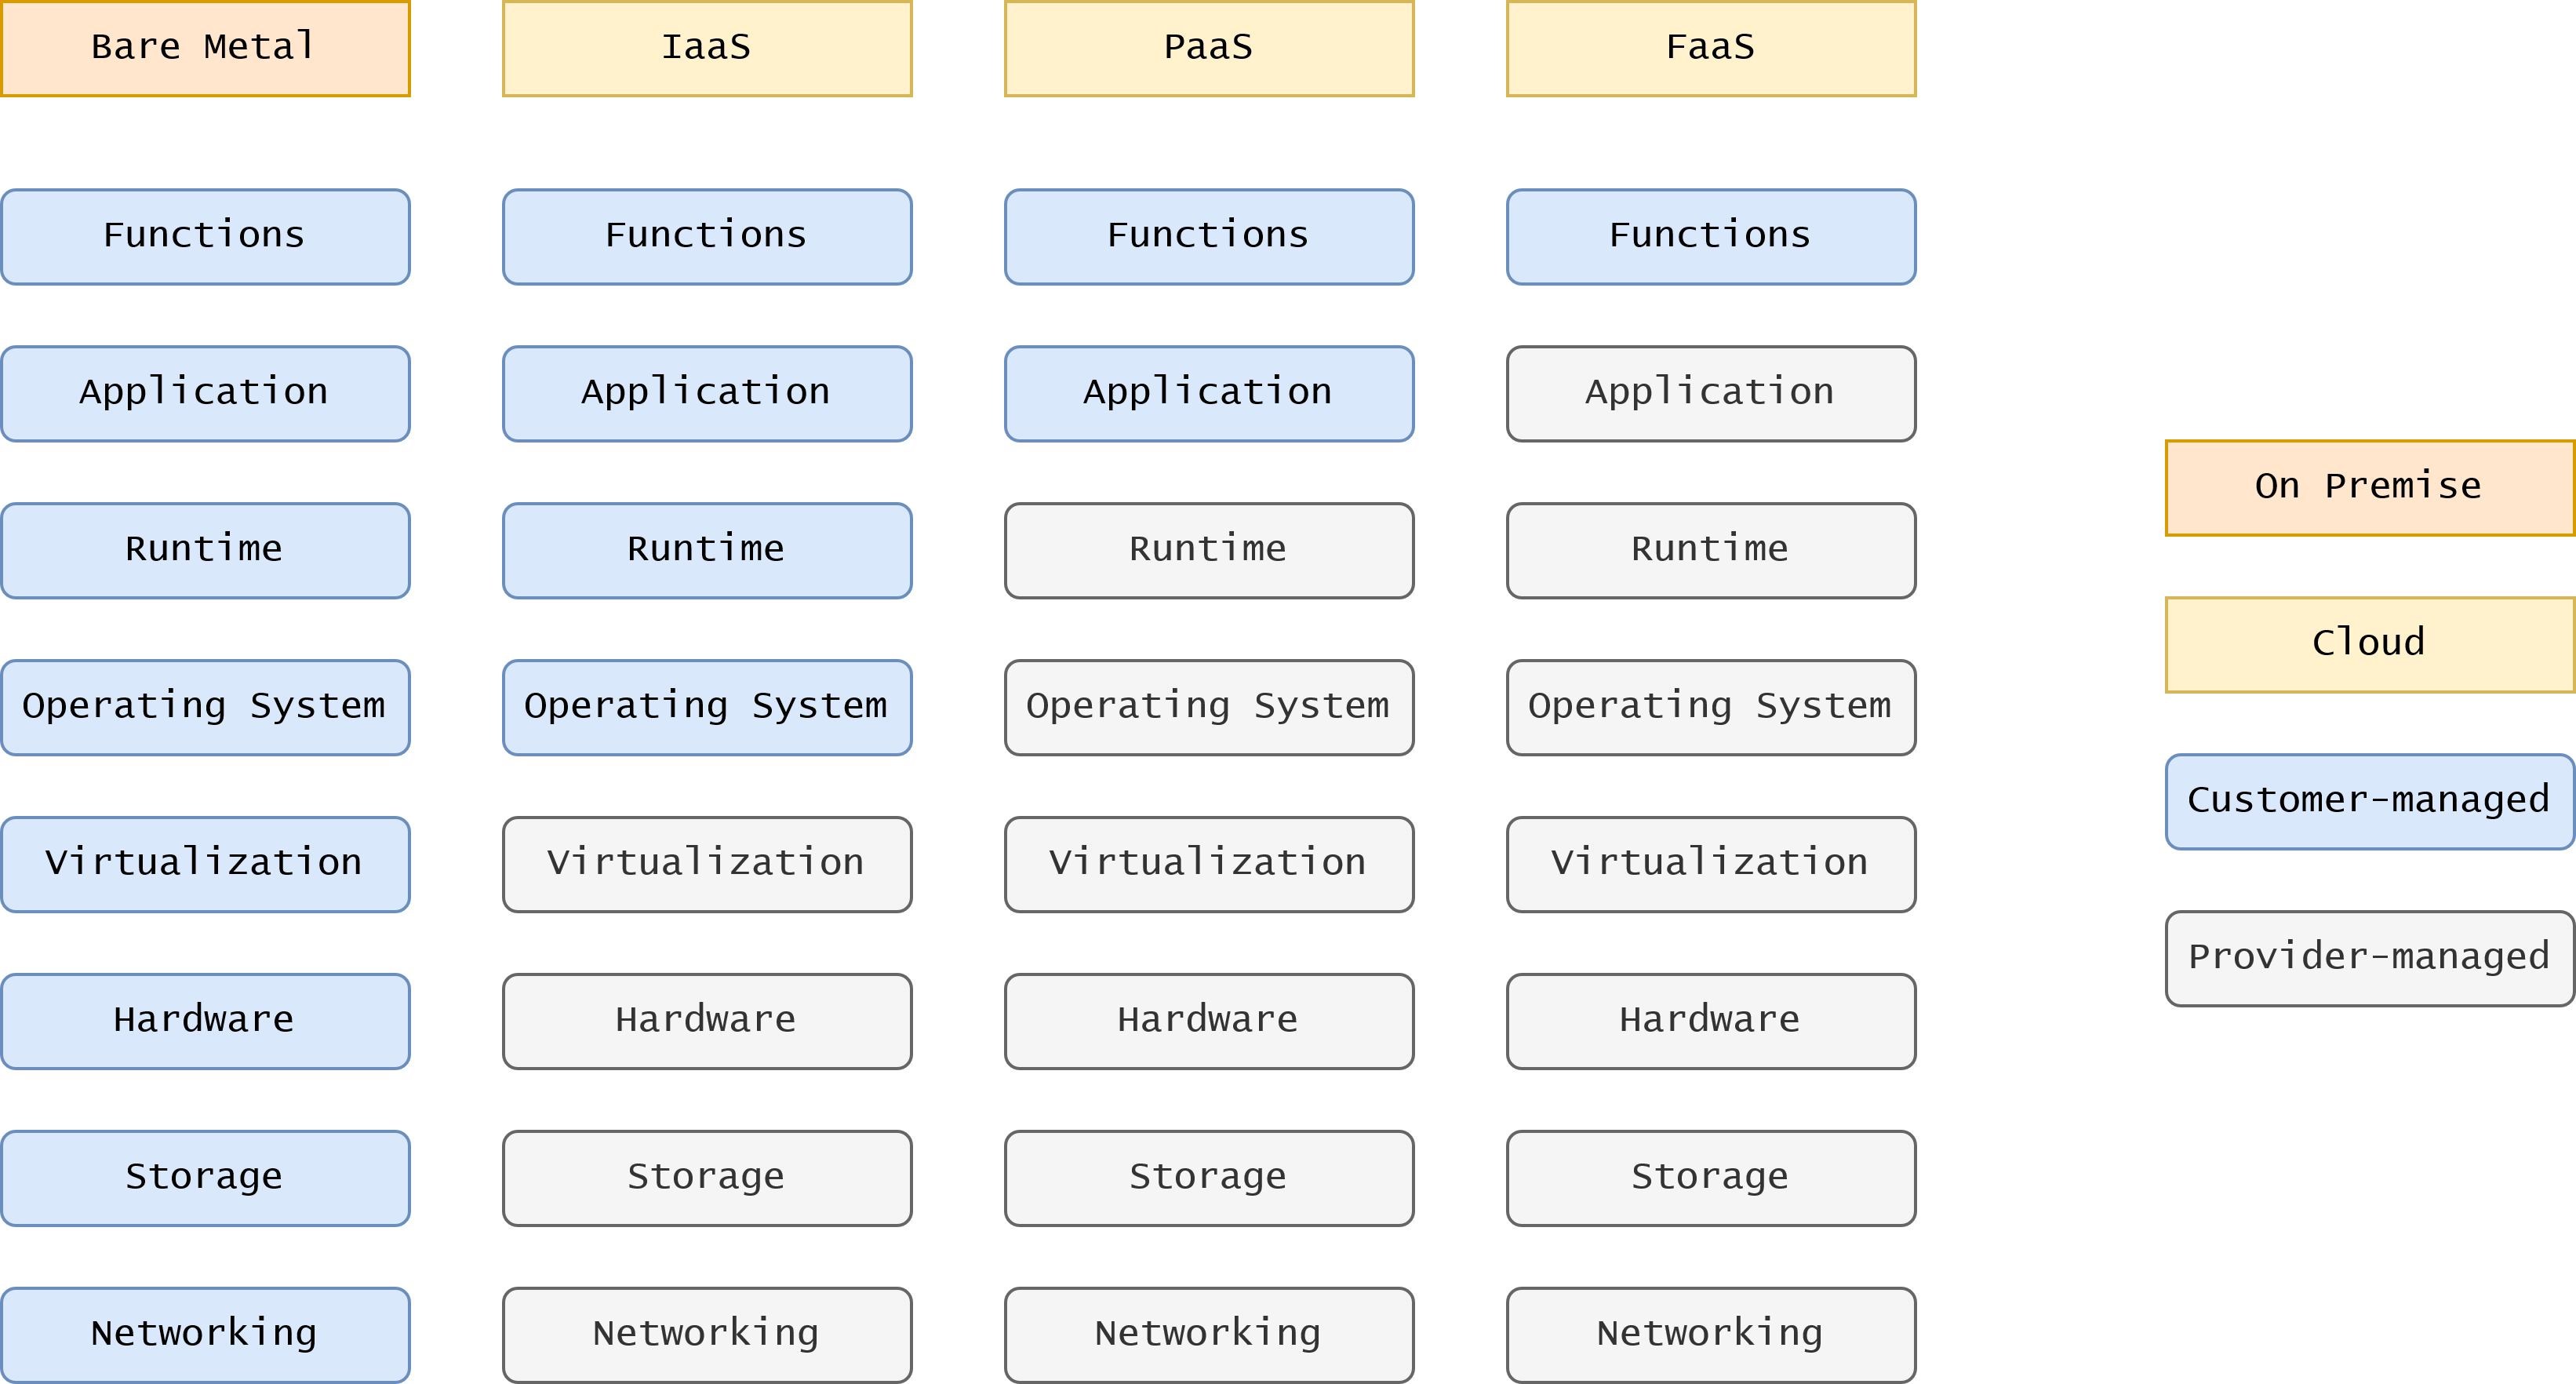
\includegraphics[width=\textwidth]{3_Chapitre1/figures/service-models.png}
	\caption[Comparaison entre différents modèles de service pour le cloud en termes de responsabilités pour le client et le fournisseur de service.]{Comparaison entre différents modèles de service pour le cloud en termes de responsabilités pour le client et le fournisseur de service (inspiré de la documentation Red Hat \protect \footnotemark).}
	\label{fig:service-model}
\end{figure}

\footnotetext{\url{https://www.redhat.com/en/topics/cloud-computing/iaas-vs-paas-vs-saas}}

Ces caractéristiques sont déclinées dans trois modèles de service, comme illustré par la figure~\ref{fig:service-model}, qui constituent des déclinaisons de l'offre commerciale des fournisseurs de service cloud :

\begin{itemize}
    \item \textbf{Software as a Service} (SaaS) -- Cible l'utilisateur final en offrant l'accès à une application entièrement administrée par le fournisseur de services ;
    \item \textbf{Platform as a Service} (PaaS) -- Cible les clients qui souhaitent déployer leurs applications sans avoir la responsabilité d'administration des serveurs ;
    \item \textbf{Infrastructure as a Service} (IaaS) -- Cible les clients qui souhaitent un contrôle à grain fin sur leurs infrastructures. Les clients d'une offre IaaS sont responsables de l'administration de leurs serveurs, souvent virtuels. 
\end{itemize}

\subsection{Modèles de déploiement}

Il existe plusieurs topologies dans le cloud, qui correspondent à différentes contraintes métier pour les utilisateurs :

\begin{itemize}
    \item \textbf{Cloud privé} -- L'infrastructure est dédiée à une organisation qui regroupe plusieurs utilisateurs finaux. Ce modèle de déploiement est privilégié pour la sécurité et la confidentialité des données ;
    \item \textbf{Cloud public} -- L'infrastructure est partagée entre de nombreux clients hétérogènes, professionnels comme particuliers ;
    \item \textbf{Cloud communautaire} -- L'infrastructure est partagée entre différents acteurs ayant souvent des problématiques métier similaires (secteurs bancaire ou hospitalier par exemple) ;
    \item \textbf{Cloud hybride} -- Solution de répartition des tâches entre cloud privé et cloud public, en fonction de leur niveau de criticité.
\end{itemize}

\subsection{La promesse du cloud computing}

Dans les faits, l'élasticité rapide, considérée par le NIST comme une caractéristique essentielle du cloud, au sens de mise à l'échelle dynamique des ressources en adéquation avec les besoins des applications déployées, n'est pas une caractéristique des offres traditionnelles dans le cloud~\cite{herbstElasticityCloudComputing}. Il incombe aux développeurs de planifier à l'avance et de spécifier leurs besoins, c'est-à-dire de réserver une quantité adéquate de ressources. Ces ressources sont généralement appelées "instances" par les fournisseurs de services cloud. Les instances cloud se distinguent généralement en fonction de leurs spécifications en termes de type de ressources et de capacité : par exemple, on peut trouver des instances avec de nombreux cœurs CPU, tandis que d'autres donnent accès à un GPU ou à un autre accélérateur matériel.

Le choix du ou des types d'instances et de leur quantité pour une application dépend a) de la nature des calculs effectués, et b) de la latence acceptable et du débit souhaité~\cite{yallesRISCLESSReinforcementLearning}. Il est de la responsabilité du client de ne pas surprovisionner au-delà de ses besoins réels.

Cette conception de l'offre a d'autres conséquences. Tout d'abord, cela signifie que la facturation est faite à gros grain : par instances réservées, plutôt que par ressources réellement utilisées. En outre, le coût des ressources inactives incombe au client. Lorsque l'application déployée ne traite aucune requête, elle reste dans un état dormant, en attente d'une nouvelle demande entrante.

Les plateformes cloud doivent prendre en charge un nombre important de traitements, ce qui entraîne une situation massivement multi-tenant qui nécessite des techniques d'isolation et de virtualisation adéquates. Celles-ci sont présentées dans la section suivante.

\section{Ordonnancement dans le cloud}

\subsection{Virtualisation dans un cadre multi-tenant}

Le cadre multi-tenant est une caractéristique déterminante du cloud. Il s'agit de la capacité d'un fournisseur de services cloud à partager des ressources entre plusieurs clients afin de réaliser des économies~\cite{weissmanDesignForceCom2009}. Comme les ressources sont mises en commun et que différentes applications les utilisent, cela ouvre des canaux, auxiliaires ou non, entre les processus dans l'espace utilisateur~\cite{pedersen2017trash, wu2018side}. Bénéficier du cadre multi-tenant s'accompagne donc de la responsabilité, pour le fournisseur, de garantir la confidentialité et la sécurité des données et des différentes charges de travail des clients~\cite{vaqueroLockingSkySurvey2011}.

Pour respecter ces garanties, les fournisseurs doivent recourir à des mesures de protection pour assurer le cloisonnement entre différents processus appartenant à des applications et/ou des utilisateurs différents. Ce mécanisme consistant à présenter, de manière transparente, un environnement d'exécution distinct avec un espace d'adressage, un système de fichiers et des autorisations propres à chaque processus est appelé isolation~\cite{fehlingCloudComputingPatterns2014}. À cette fin, les fournisseurs peuvent s'appuyer sur des technologies de virtualisation.

La virtualisation est une technique d'isolation qui permet d'exécuter une application dans les limites d'un environnement d'exécution sécurisé, appelé \textit{sandbox}, en introduisant une couche d'indirection entre la plateforme hôte et l'application elle-même~\cite{singhviAtollScalableLowLatency2021}.

La virtualisation des ressources de l'hôte peut se faire à l'aide de machines virtuelles (VM) ou de conteneurs. Ces environnements d'exécution donnent aux processus sous-jacents l'illusion d'avoir une machine entière à leur disposition. Alors que les VM virtualisent les ressources physiques de l'hôte, en s'appuyant sur l'architecture du processeur pour réaliser l'isolation, les conteneurs exploitent des directives du système d'exploitation hôte pour isoler les charges de travail~\cite{mancoMyVMLighter2017}.

Ces techniques sont bénéfiques à la fois du côté du fournisseur et du côté du développeur. Le premier tire parti de la virtualisation pour isoler les charges de travail des clients, et exploite la flexibilité des VM pour gérer leur mise à l'échelle compte tenu d'une quantité finie de ressources matérielles. Les seconds organisent leur infrastructure de manière à reproduire un environnement de type production pendant les phases de développement, ainsi que pour livrer et déployer leurs produits.

La virtualisation est devenue une telle pierre angulaire des services cloud que Kubernetes~\cite{kubernetes}, un système d'orchestration qui s'appuie sur des conteneurs\footnote{On note que Kubevirt~\cite{kubevirt} vise à adapter Kubernetes au déploiement de VM.} pour gérer le cycle de vie des applications, de leur déploiement à leur mise à l'échelle, est de plus en plus souvent appelé "le système d'exploitation pour le cloud"~\cite{jonreeve2018kubernetes}.

Lorsqu'ils choisissent le modèle d'isolation sur lequel ils souhaitent s'appuyer pour exploiter le partage des ressources, les fournisseurs cloud doivent faire un compromis entre performances et sécurité. Les conteneurs sont fréquemment la cible d'attaques par élévation de privilèges~\cite{zomer2022containers, redhat2019containers}, mais leurs performances sont de plusieurs ordres de grandeur supérieures à celles des machines virtuelles : le temps de démarrage des conteneurs se compte en centaines de millisecondes, tandis que les VM démarrent en quelques secondes~\cite{mancoMyVMLighter2017}. La conception de machines virtuelles légères offrant des performances comparables à celles des conteneurs est un sujet de recherche essentiel~\cite{agacheFirecrackerLightweightVirtualization, Anjali2020BlendingCA}).

\begin{figure}[htbp]
    \centering
	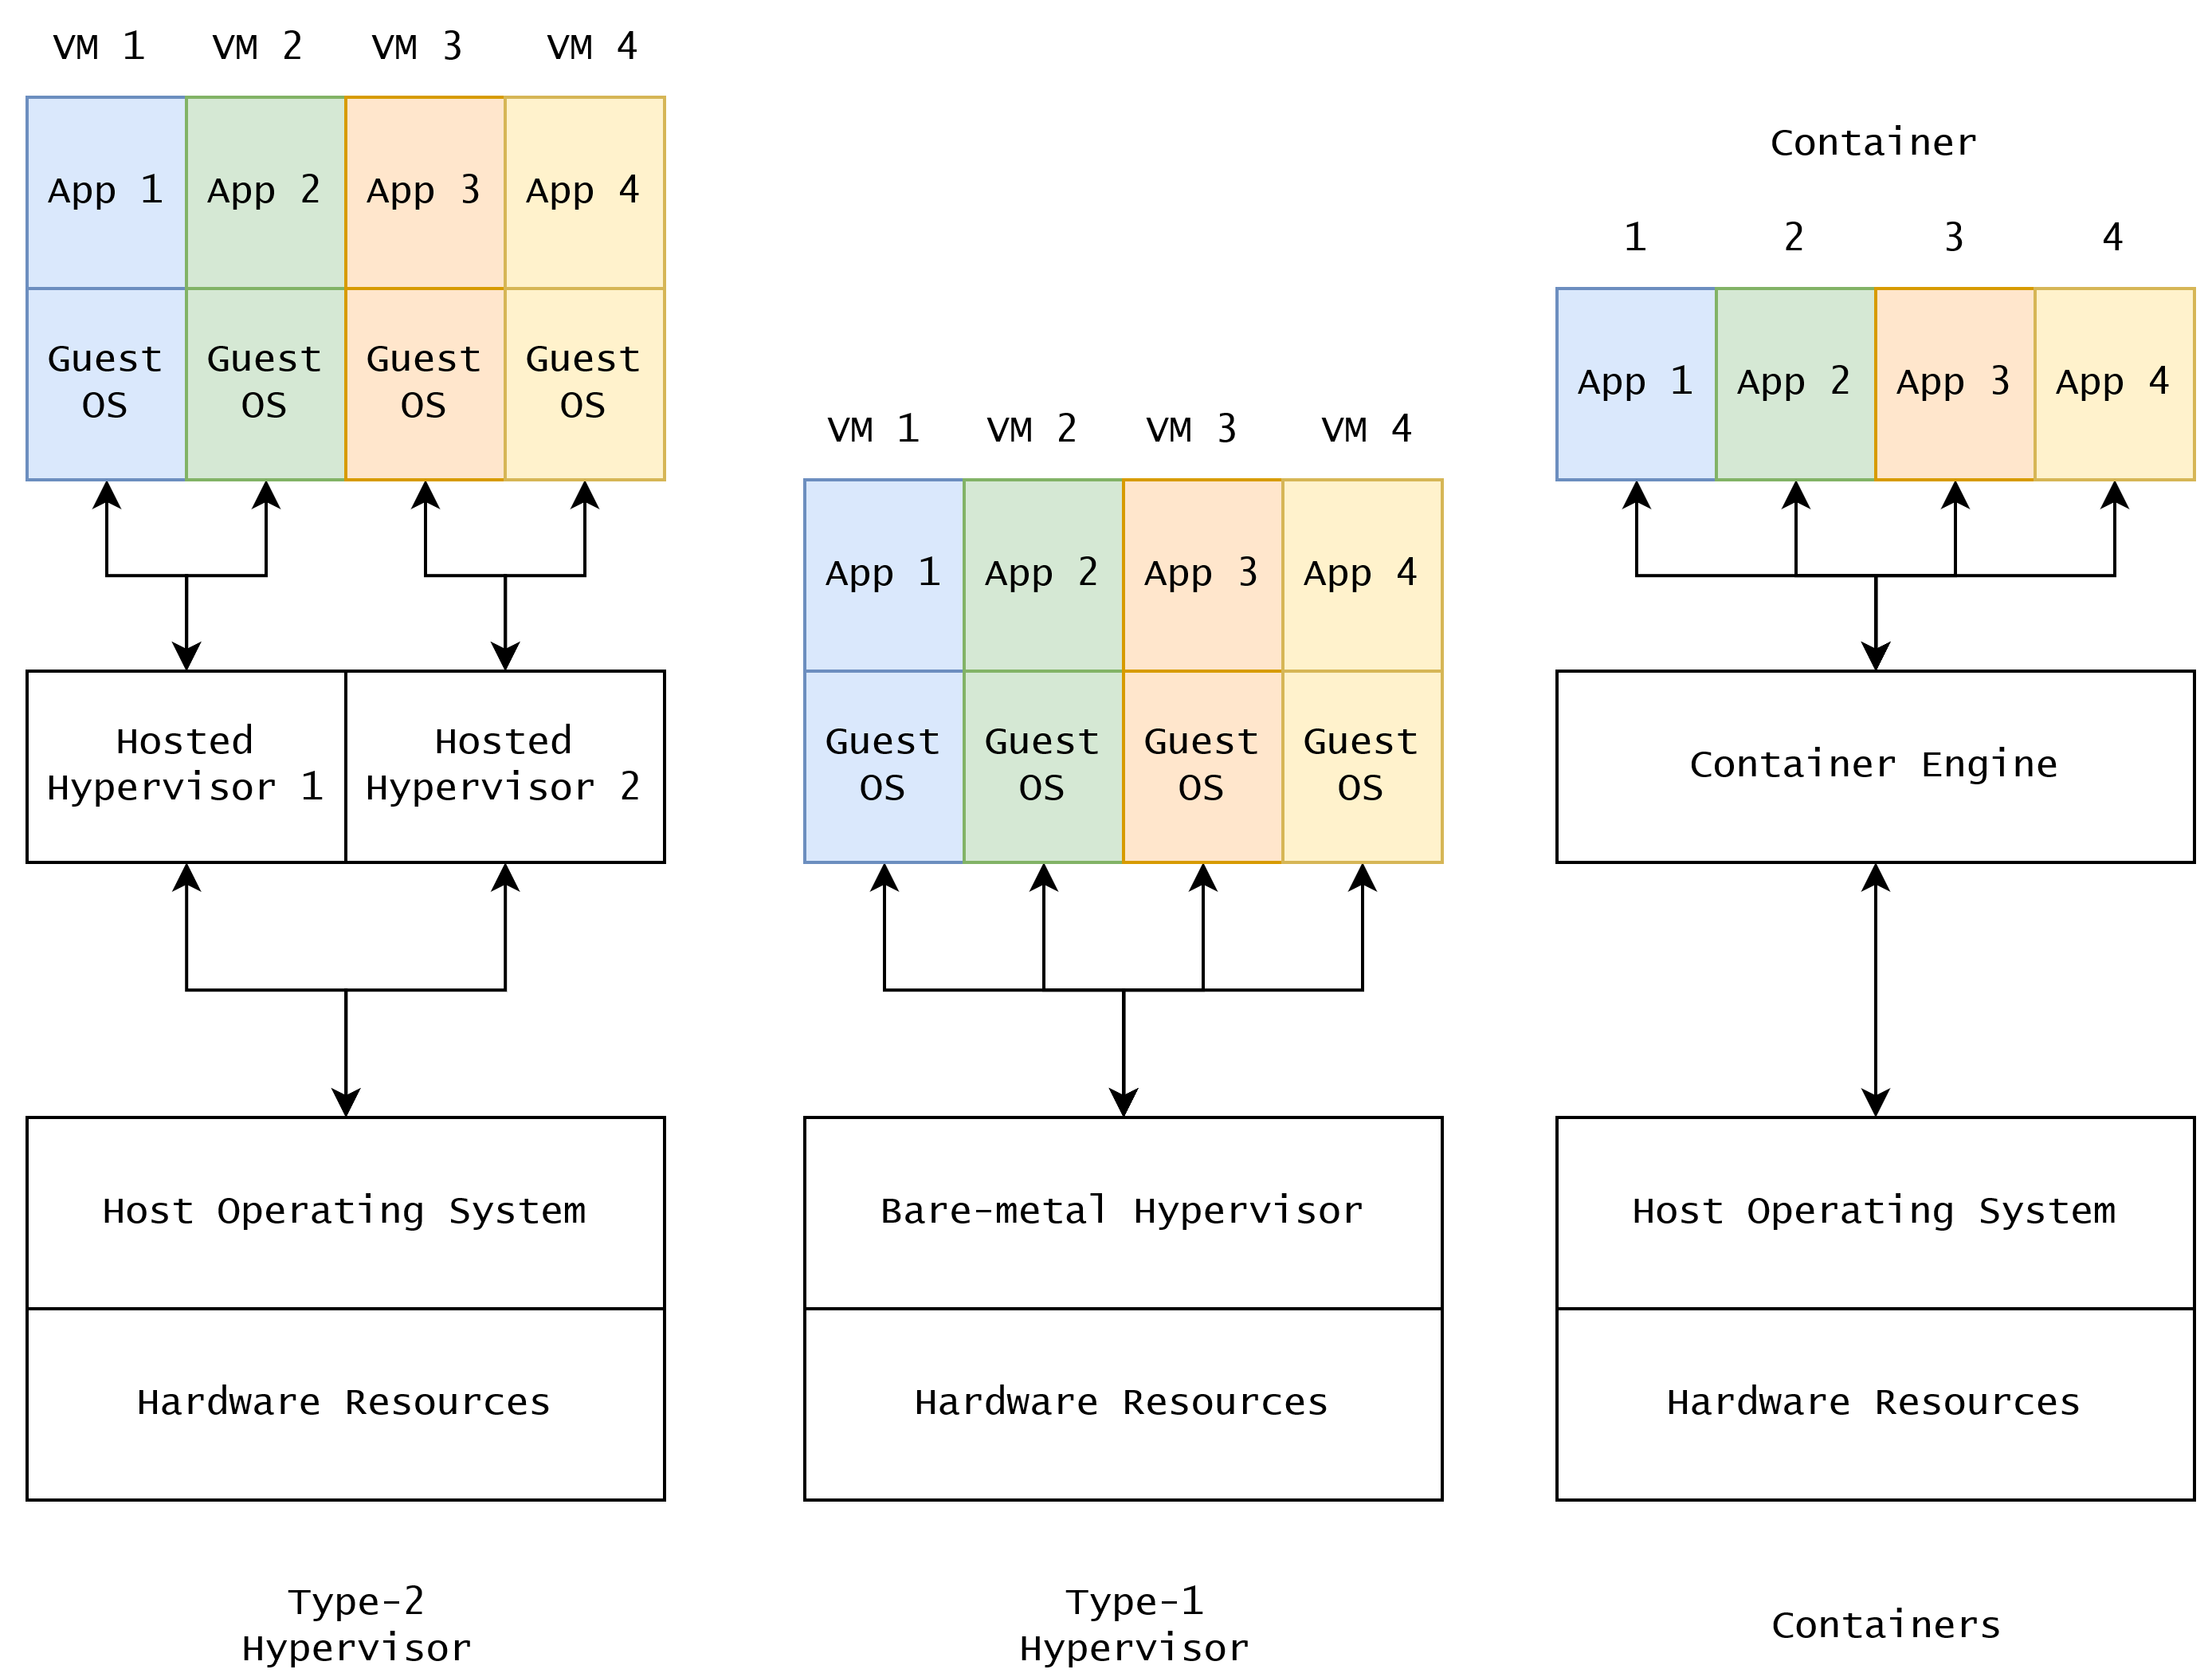
\includegraphics[width=\textwidth]{3_Chapitre1/figures/virtualization.png}
	\caption{Aperçu des différents modèles d'isolation : virtualisation et conteneurisation.}
	\label{fig:virtualization}
\end{figure}

\subsubsection{Machines virtuelles}

Les machines virtuelles virtualisent les ressources physiques de l'hôte : la virtualisation assistée par le matériel permet à plusieurs systèmes d'exploitation \textit{invités} complets de fonctionner indépendamment sur des ressources physiques partagées, quelle que soit la nature du système d'exploitation \textit{hôte}~\cite{kivityKvmLinuxVirtual}.

Du point de vue d'une VM, son environnement d'exécution isolé est perçu comme une plateforme complète, alors qu'il s'agit en réalité d'un sous-ensemble des ressources de la plateforme hôte, déterminé par l'hyperviseur (ou VMM pour Virtual Machine Manager), un logiciel de bas niveau qui peut s'exécuter sur du \textit{bare-metal} ou en tant que processus du système d'exploitation hôte.

L'hyperviseur a la responsabilité de gérer le cycle de vie des machines virtuelles : la création, l'exécution, la destruction et parfois la migration des machines virtuelles sont gérées par l'hyperviseur.

Les hyperviseurs existent sous deux formes différentes, comme le montre la figure~\ref{fig:virtualization} :

\begin{itemize}
    \item Les hyperviseurs de type 1 (bare-metal) s'exécutent directement sur le matériel de la machine hôte. Étant donné qu'ils ne dépendent pas d'un système d'exploitation sous-jacent, ils sont considérés comme plus sûrs et plus efficaces que leurs homologues hébergés. Parmi les exemples courants d'hyperviseurs de type 1, citons VMware ESXi~\cite{esxi}, KVM~\cite{kvm}, Xen~\cite{xen} et Hyper-V~\cite{hyper-v} ;
    \item Les hyperviseurs de type 2 (hébergés) s'exécutent au-dessus d'un système d'exploitation. Ces hyperviseurs sont des produits grand public qui offrent aux utilisateurs finaux un moyen pratique d'exécuter des systèmes ou des programmes qui ne seraient pas pris en charge par leur matériel ou leur système d'exploitation. Parmi les hyperviseurs de type 2, citons QEMU~\cite{qemu} et Oracle VirtualBox~\cite{virtualbox}.
\end{itemize}

\subsubsection{Conteneurs}

La conteneurisation est une technique de virtualisation au niveau du système d'exploitation. Le noyau du système d'exploitation hôte est responsable de l'allocation des ressources. Les conteneurs virtualisent le système d'exploitation : ils donnent au processus conteneurisé l'impression d'avoir toute la machine à leur disposition, tout en étant en réalité contraint et limité en ce qui concerne l'utilisation des ressources par le noyau hôte~\cite{bentalebContainerizationTechnologiesTaxonomies2022}.

Du point de vue de l'application en cours d'exécution, la plateforme d'exécution se comporte comme s'il s'agissait de bare-metal. Toutefois, les ressources qui lui sont allouées sont en fait un sous-ensemble virtualisé des ressources matérielles de l'hôte.

Les conteneurs constituent un mécanisme d'isolation léger qui repose sur les capacités d'isolation du noyau du système hôte, comme le montre la figure~\ref{fig:virtualization}. En l'occurrence, sous Linux :

\begin{itemize}
    \item \texttt{chroot} : modifie le répertoire racine apparent pour une arborescence de processus donnée. Il permet à un conteneur d'opérer sur un répertoire virtuel \texttt{/} qui pourrait être situé n'importe où sur le système de fichiers de l'hôte ;
    \item \texttt{cgroups} : permettent de créer des groupes hiérarchiques de processus et allouer, limiter et surveiller les ressources matérielles pour ces groupes : E/S vers et depuis les périphériques de bloc, accès à l'unité centrale, à la mémoire et aux interfaces réseau ;
    \item \texttt{namespaces} : une couche d'abstraction autour des ressources globales du système, telles que le réseau ou les communications entre processus (IPC). Les processus au sein d'un espace de noms ont leurs propres instances isolées de ces ressources système.
\end{itemize}

L'ambition derrière les conteneurs est de contenir l'exécution d'une application dans un processus isolé du reste du système, de sorte à ce qu'il ignore les autres processus exécutés par le système hôte. Le conteneur est amorcé à partir d'une image qui contient toutes les dépendances nécessaires à la construction et/ou à l'exécution de l'application.

Dans l'écosystème des conteneurs, Docker~\cite{docker} en particulier a connu une forte progression depuis sa création en 2013. Docker a joué un rôle déterminant dans la spécification des normes industrielles pour les formats de conteneurs et les temps d'exécution par le biais de l'Open Container Initiative (OCI)~\cite{oci}.

La spécification OCI est une initiative de la Fondation Linux~\cite{linuxfoundation} visant à concevoir une norme ouverte pour les conteneurs. Elle définit les spécifications des images de conteneurs - des lignes directrices sur la manière de créer une image OCI avec son manifeste, ses couches de système de fichiers et sa configuration - et les spécifications d'exécution concernant la manière d'exécuter les paquets d'applications au fur et à mesure qu'ils sont décompressés sur le système d'exploitation hôte.

\subsection{Dimensionnement et passage à l'échelle}

Lorsque la charge sur une application augmente, il existe deux façons de faire de la place pour les nouvelles requêtes en procédant à une mise à l'échelle (ou \textit{scaling}) :

\begin{itemize}
    \item \textbf{Verticalement} : en attachant plus de ressources matérielles aux serveurs qui supportent l'application (par exemple, augmenter le nombre de CPU ou la quantité de mémoire alloués). Il peut s'agir de déplacer des données vers de nouveaux serveurs plus puissants, ce qui a un impact sur la disponibilité de l'application ;
    \item \textbf{Horizontalement} : en augmentant le nombre de serveurs pour faire fonctionner l'application. Cela peut signifier l'introduction d'un mécanisme d'équilibrage de la charge pour acheminer les requêtes et les réponses entre les utilisateurs et les multiples instances d'une application, ce qui a un impact sur la complexité du déploiement.
\end{itemize}

L'opération contraire peut être symétrique, ou non, lorsque le nombre ou la complexité des traitements diminue.

\subsection{Qualité de service et métriques de performances}

Problème : overbooking, overcommitting... conso d'énergie...

TODO: Consommation d'énergie, niveaux d'usage des ressources < 15\% assez classiques~\cite{vasanWorthTheirWatts2010, vermaLargescaleClusterManagement2015a} pour absorber les pannes et les interférences entre workloads. PUE moyen en 2022 autour de 1.55~\cite{davisUptimeInstituteGlobal2022}

\section{Applications dans le cloud}

\subsection{Du monolithe aux micro-services}

Le cloud computing a vu naître de nouvelles techniques de développement. Le développement "cloud-native" consiste à construire des applications pour le cloud dès le départ, en prenant en compte dès leur conception les besoins futurs de mise à l'échelle~\cite{dragoniMicroservicesHowMake2018, martinfowler2014microservices}.

Une application monolithique est construite comme une unité unique. Il n'y a pas de découplage entre les services qu'elle expose, car ils font tous partie de la même base de code~\cite{villamizarEvaluatingMonolithicMicroservice2015}. Lors de la mise à l'échelle d'un monolithe, l'ajout de ressources supplémentaires (mise à l'échelle verticale) ne résout pas le problème des priorités concurrentes au sein de l'application : lorsque la popularité d'une application monolithique augmente, certaines parties de la base de code seront sollicitées plus que d'autres, mais la pression ne sera pas répartie sur l'ensemble de l'application. D'autre part, l'augmentation du nombre d'instances du monolithe (mise à l'échelle horizontale) peut s'avérer inefficace en termes de coûts, car toutes les parties d'une application ne subissent pas des pics de charge en même temps : dans la figure \ref{fig:scaling-monolith}, une augmentation des requêtes d'authentification implique une mise à l'échelle de l'infrastructure pour l'ensemble de l'application.

\begin{figure}[ht]
    \centering
	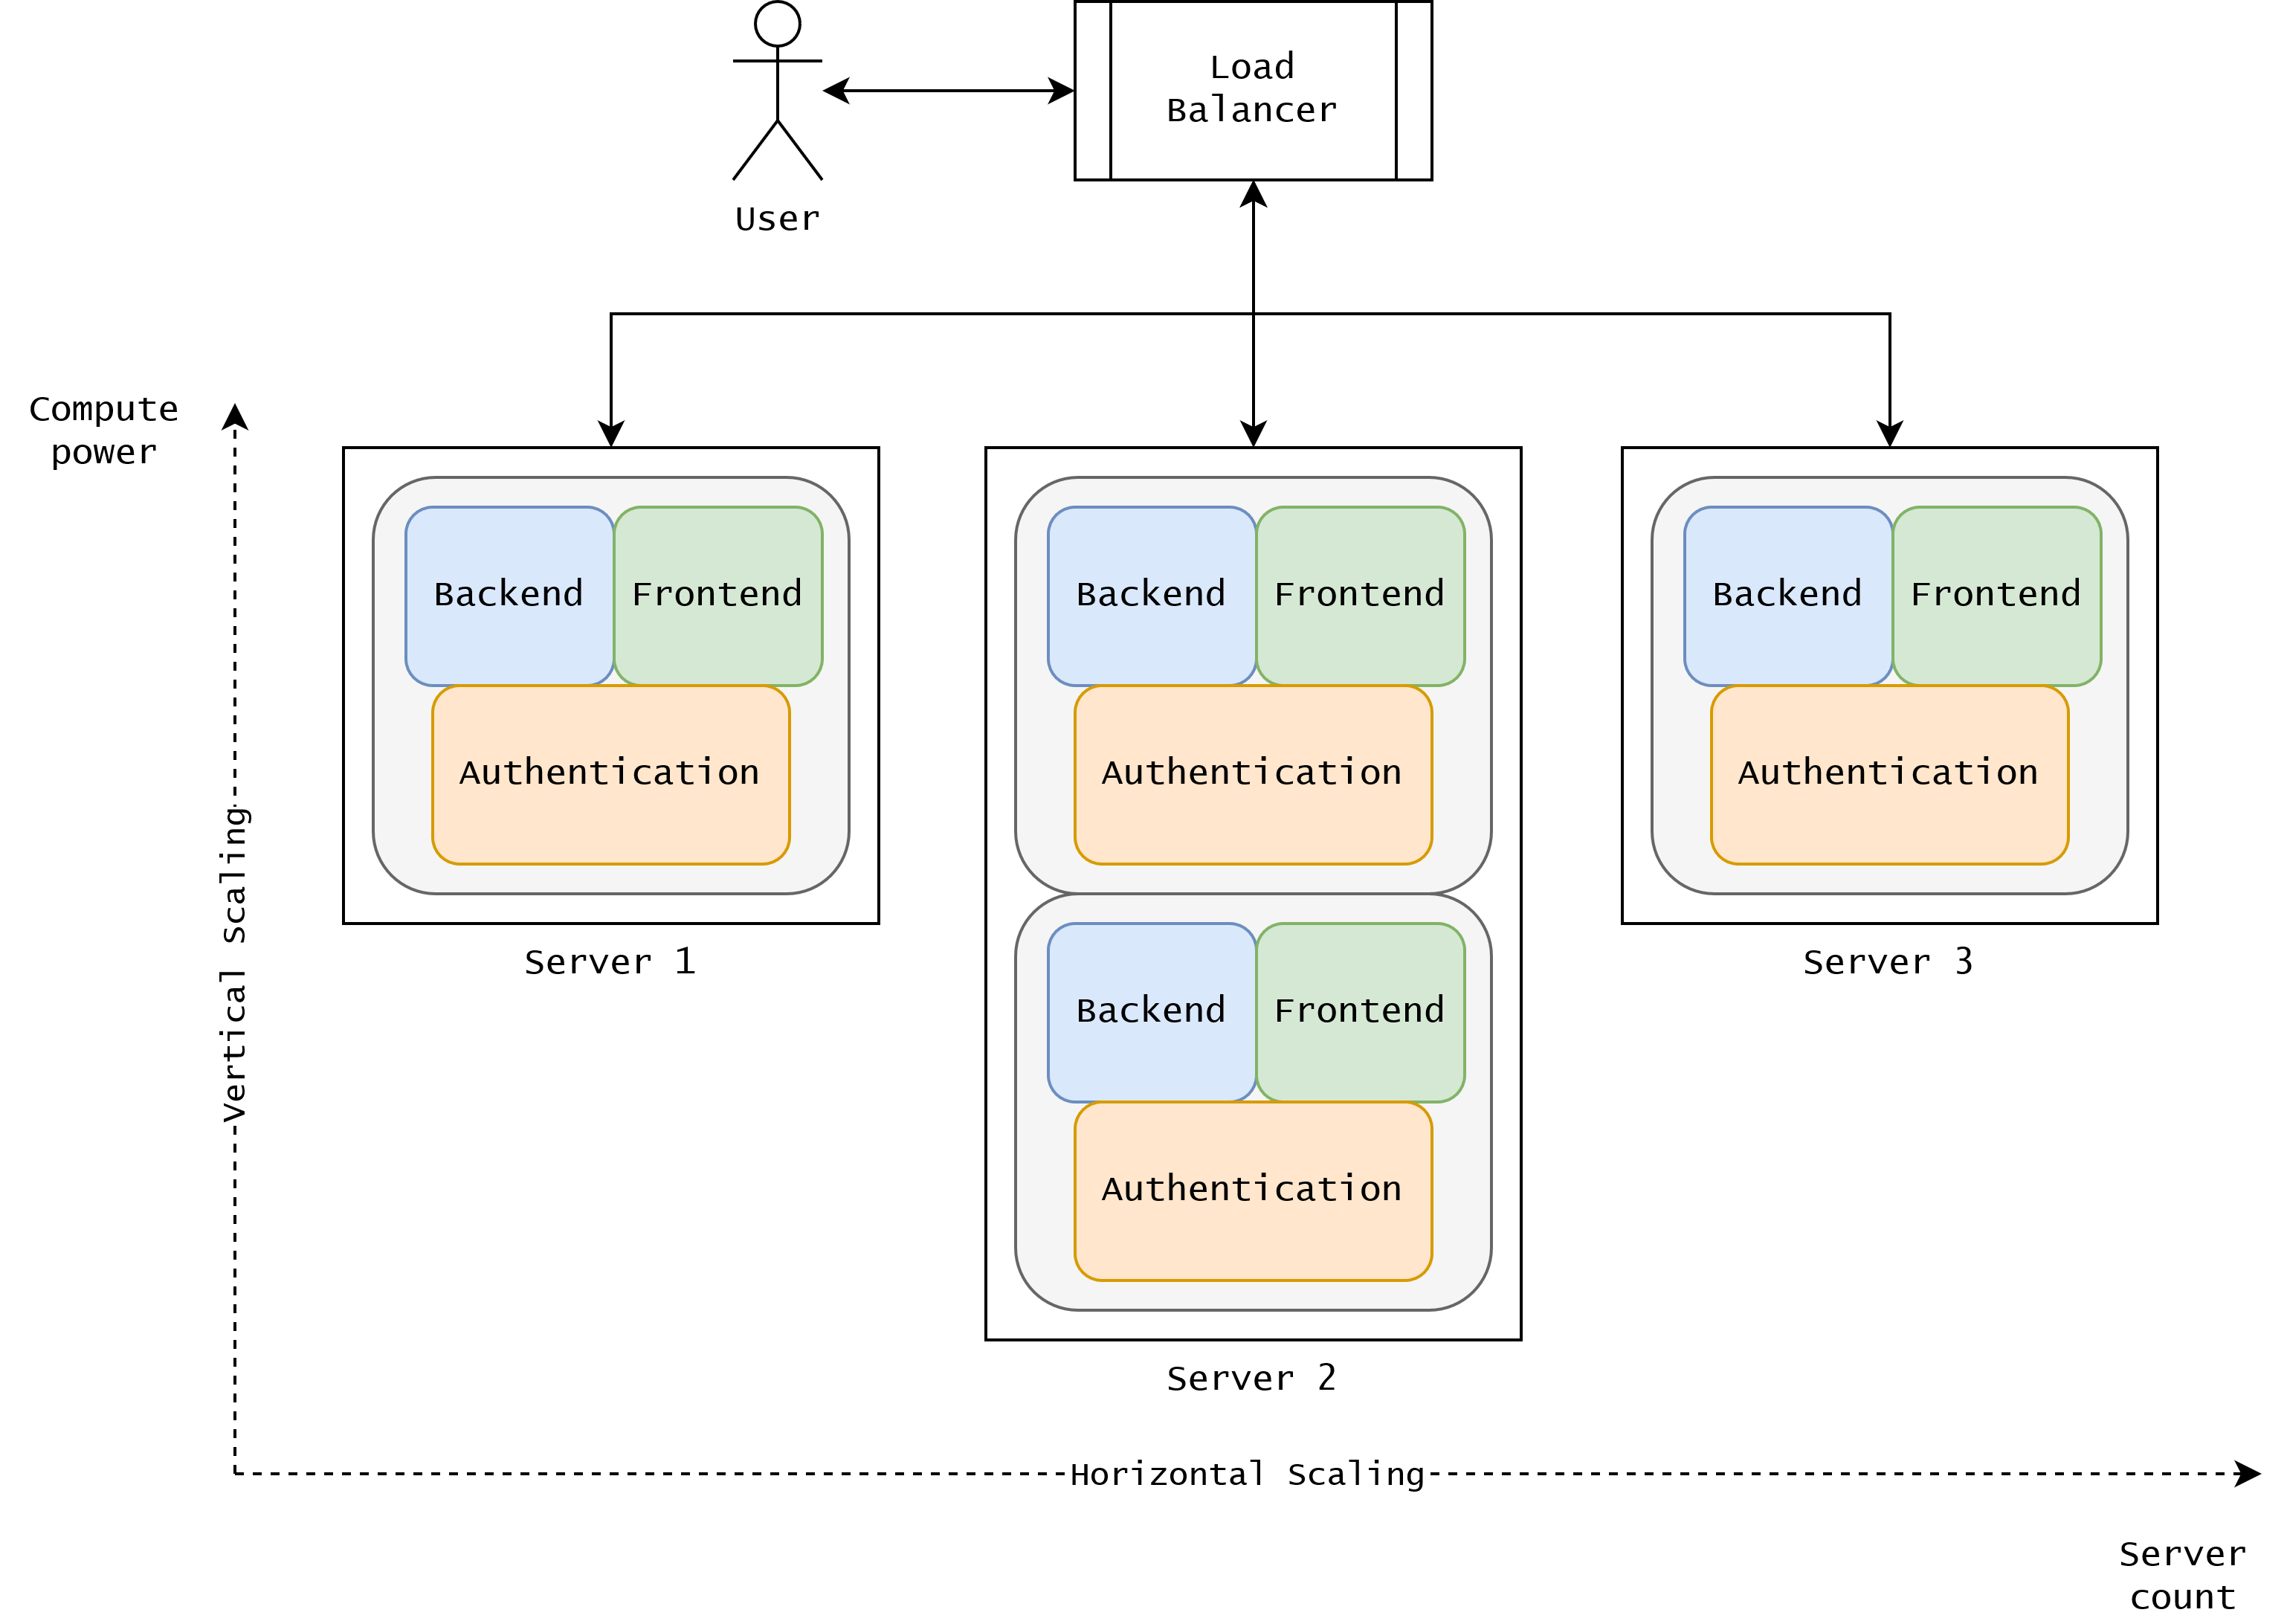
\includegraphics[width=\textwidth]{3_Chapitre1/figures/scaling-monolith.png}
	\caption{La mise à l'échelle d'une application à architecture monolithique nécessite de répliquer le monolithe sur plusieurs serveurs.}
	\label{fig:scaling-monolith}
\end{figure}

La méthodologie Twelve-Factor App, un ensemble de lignes directrices pour la création d'applications cloud-natives, recommande "[d'exécuter] l'application sous la forme d'un ou plusieurs processus sans état"~\cite{12factor}. C'est ce qu'on appelle une architecture de microservices, qui consiste à organiser une application sous la forme d'une collection de services faiblement couplés. Chacun de ces services s'exécute dans son propre processus, communique avec les autres par le biais du passage de messages et peut être déployé de manière indépendante sur des serveurs hétérogènes afin d'atteindre les objectifs de niveau de service : dans la figure \ref{fig:scaling-microservices}, une augmentation des requêtes d'authentification peut être absorbée par la mise à l'échelle de l'infrastructure pour le seul microservice d'authentification.

\begin{figure}[ht]
    \centering
	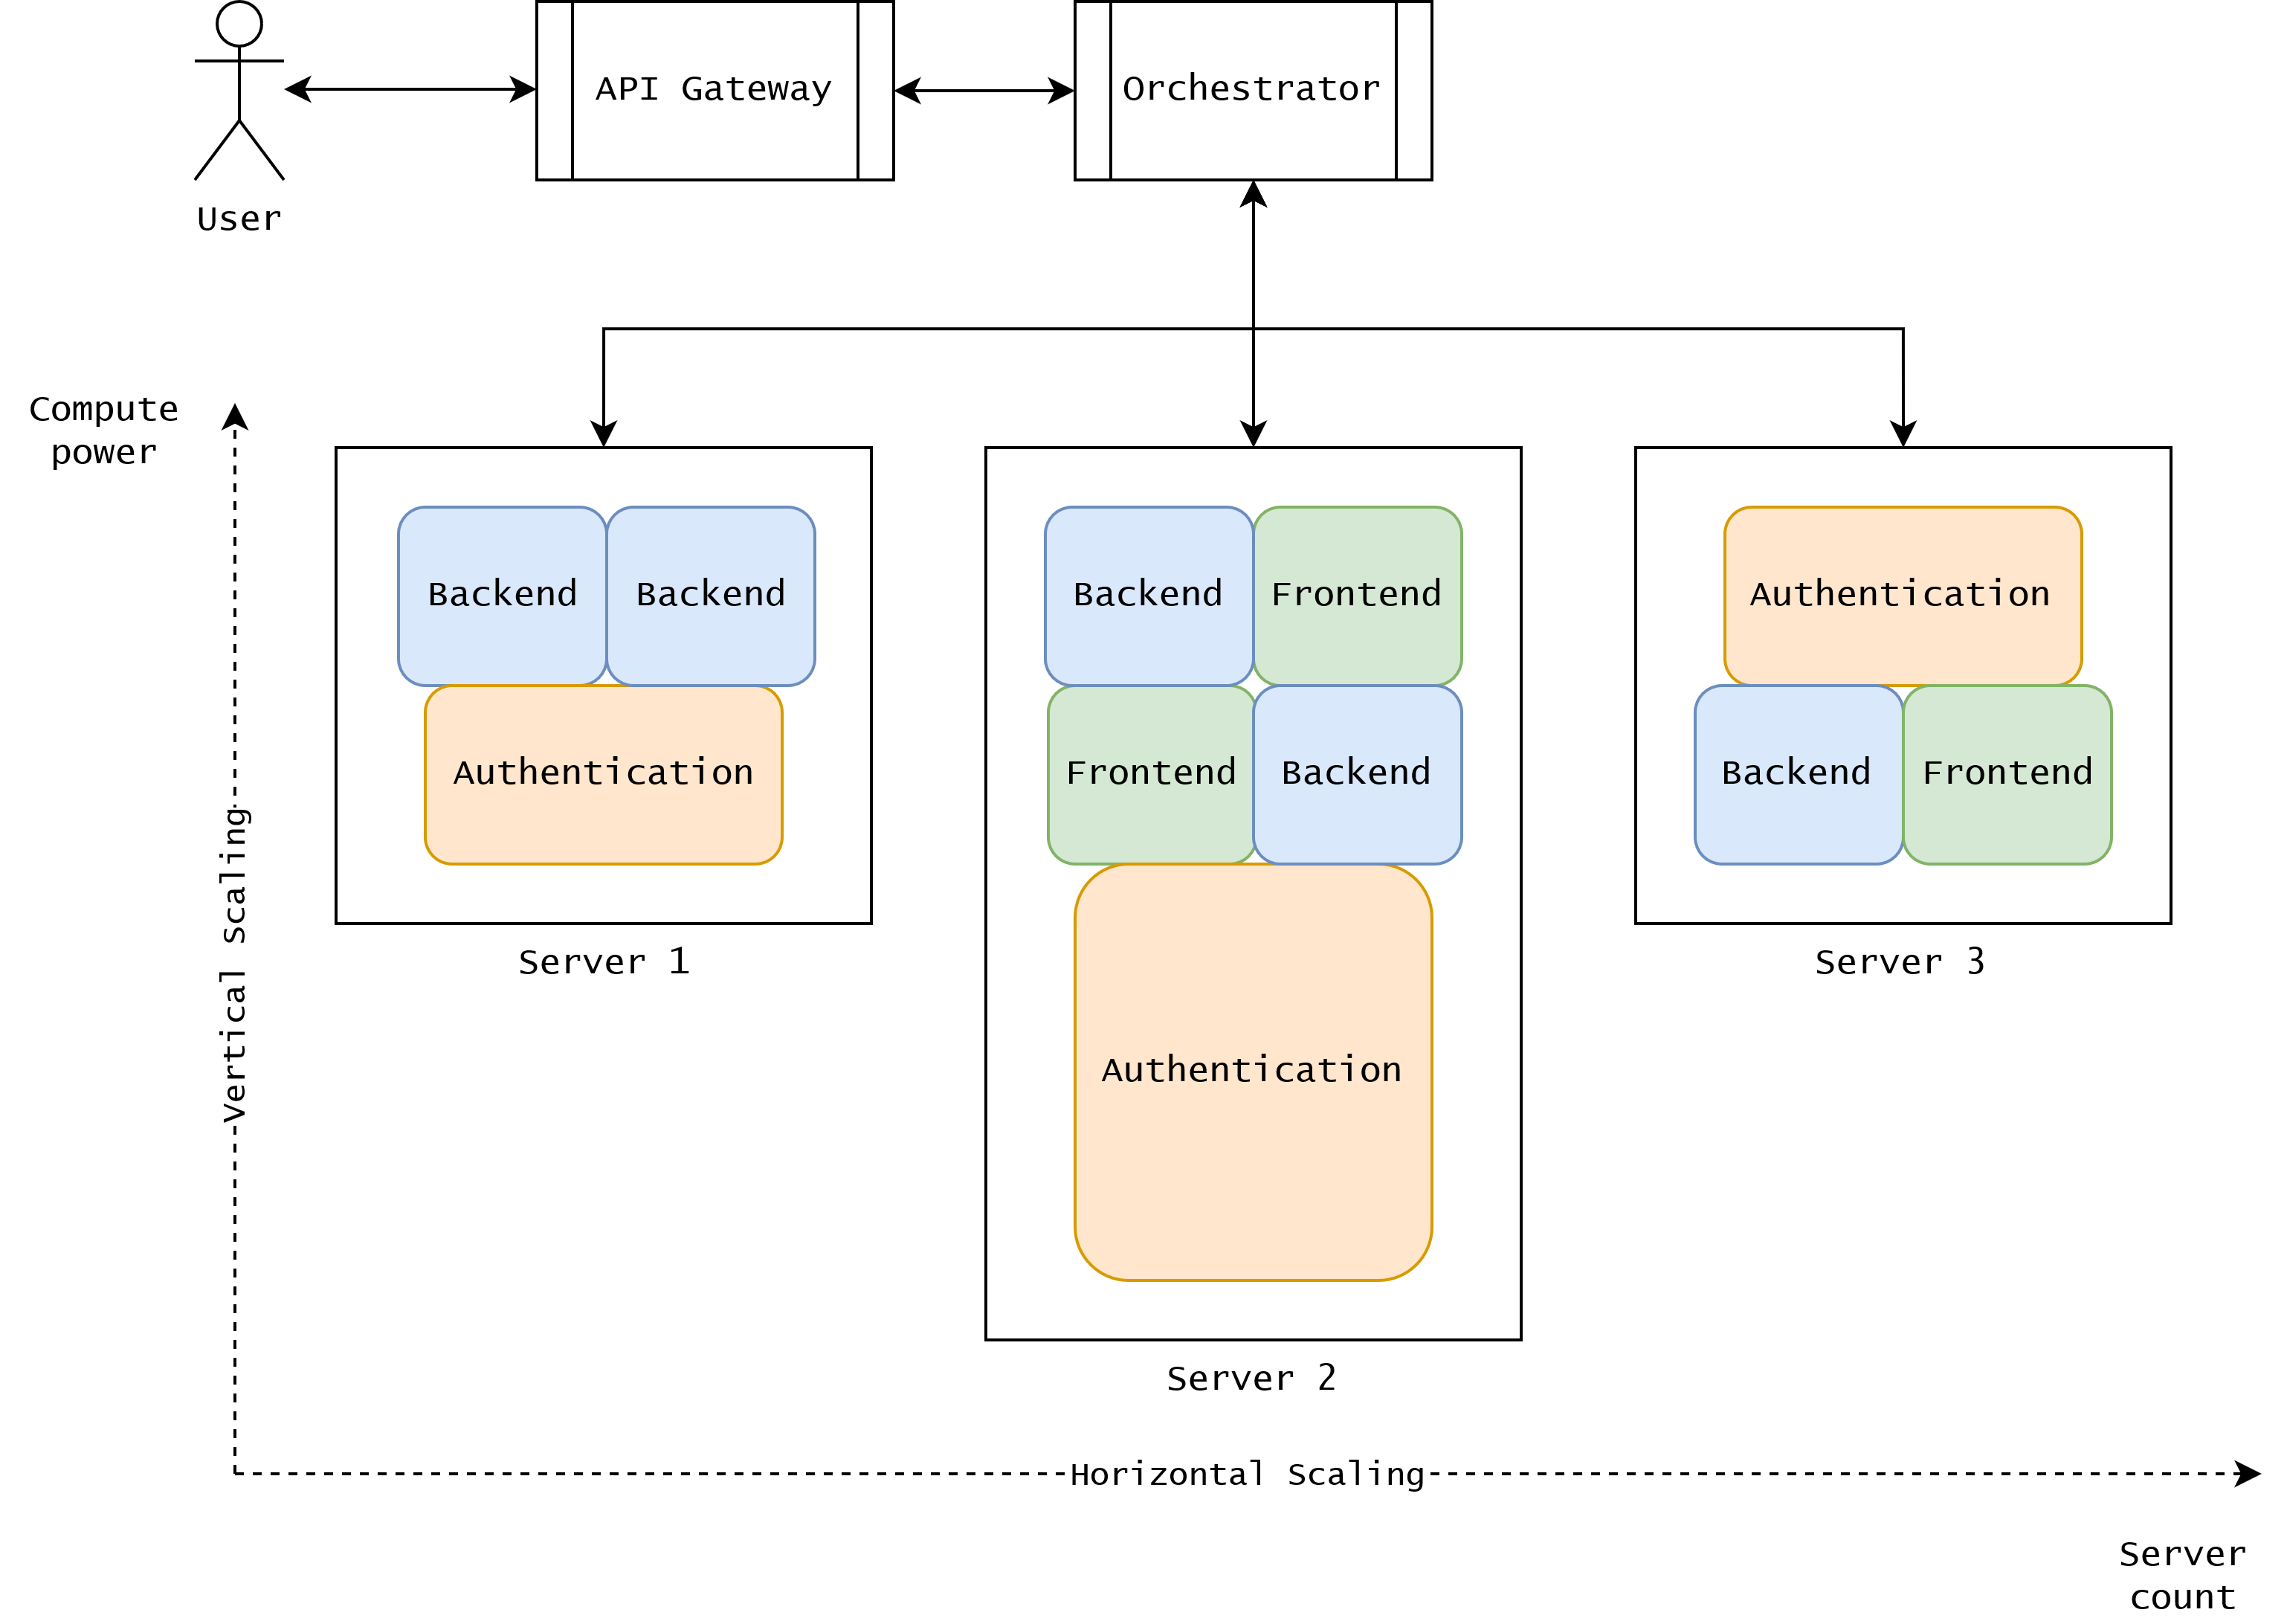
\includegraphics[width=\textwidth]{3_Chapitre1/figures/scaling-microservices.png}
	\caption{La mise à l'échelle d'une application architecturée en microservices permet de distribuer et de répliquer chaque microservice de manière indépendante.}
	\label{fig:scaling-microservices}
\end{figure}

Toutefois, une infrastructure de microservices implique une couche complexe de gestion centralisée, qui entraîne des coûts dans les opérations ou dans les équipes DevOps. Elle repose sur des services dorsaux de longue durée (bases de données, bus de messages, etc.) qui doivent également être surveillés et gérés. Dans les environnements IaaS et PaaS, l'expérience des développeurs en particulier n'est pas satisfaisante : le déploiement du cloud s'accompagne d'un fardeau d'administration des systèmes~\cite{jonasCloudProgrammingSimplified2019}. Les microservices ne résolvent pas à eux seuls le problème du déploiement : l'écriture de recettes d'images de conteneurs n'ajoute pas de valeur au produit, car elle relève de la logique opérationnelle plutôt que de la logique commerciale.

TODO: Conclusion avec ouverture sur le serverless

\subsection{Vers un nouveau modèle de service}

Dans cette section, nous présentons le modèle serverless de programmation et de déploiement d'applications dans le cloud. Nous passerons en revue les caractéristiques essentielles des plateformes serverless et mettrons en évidence les compromis que les fournisseurs de services et les développeurs d'applications doivent prendre en compte lorsqu'ils ciblent des infrastructures serverless. Cette section propose également une description des offres serverless dans les solutions de cloud public, et des plateformes open source pour les architectes de cloud privé.

\subsubsection{Caractéristiques des plateformes serverless}

Le serverless désigne à la fois un modèle de programmation et un modèle de service pour le cloud computing. Dans une architecture serverless, les développeurs conçoivent leurs applications comme une composition de fonctions sans état. Sans état (ou "pur", sans effet de bord) signifie que le résultat du calcul dépend exclusivement des entrées~\cite{burckhardtNetheriteEfficientExecution}. Ces fonctions prennent en entrée une valeur et un contexte d'invocation, et produisent un résultat qui est stocké dans un niveau de stockage persistant. Leur exécution est déclenchée par un événement qui peut être décrit comme la notification d'un message entrant, qu'il s'agisse d'une requête HTTP, d'une tâche planifiée, d'un téléchargement de fichier, etc. Ainsi, le serverless est un modèle dirigé par les événements~\cite{SchleierSmith2021WhatSC}.

La conception susmentionnée est illustrée par un exemple d'application serverless dans la figure~\ref{fig:web-app} : lorsque la requête de l'utilisateur atteint la passerelle (ou API) de la plateforme serverless, celle-ci déclenche l'exécution de différentes fonctions selon la route HTTP demandée -- ces fonctions ne sont pas des \textit{daemons} à l'écoute d'événements (par exemple, sur un socket ouvert), elles sont exécutées à la demande.

\begin{figure}[htbp]
    \centering
	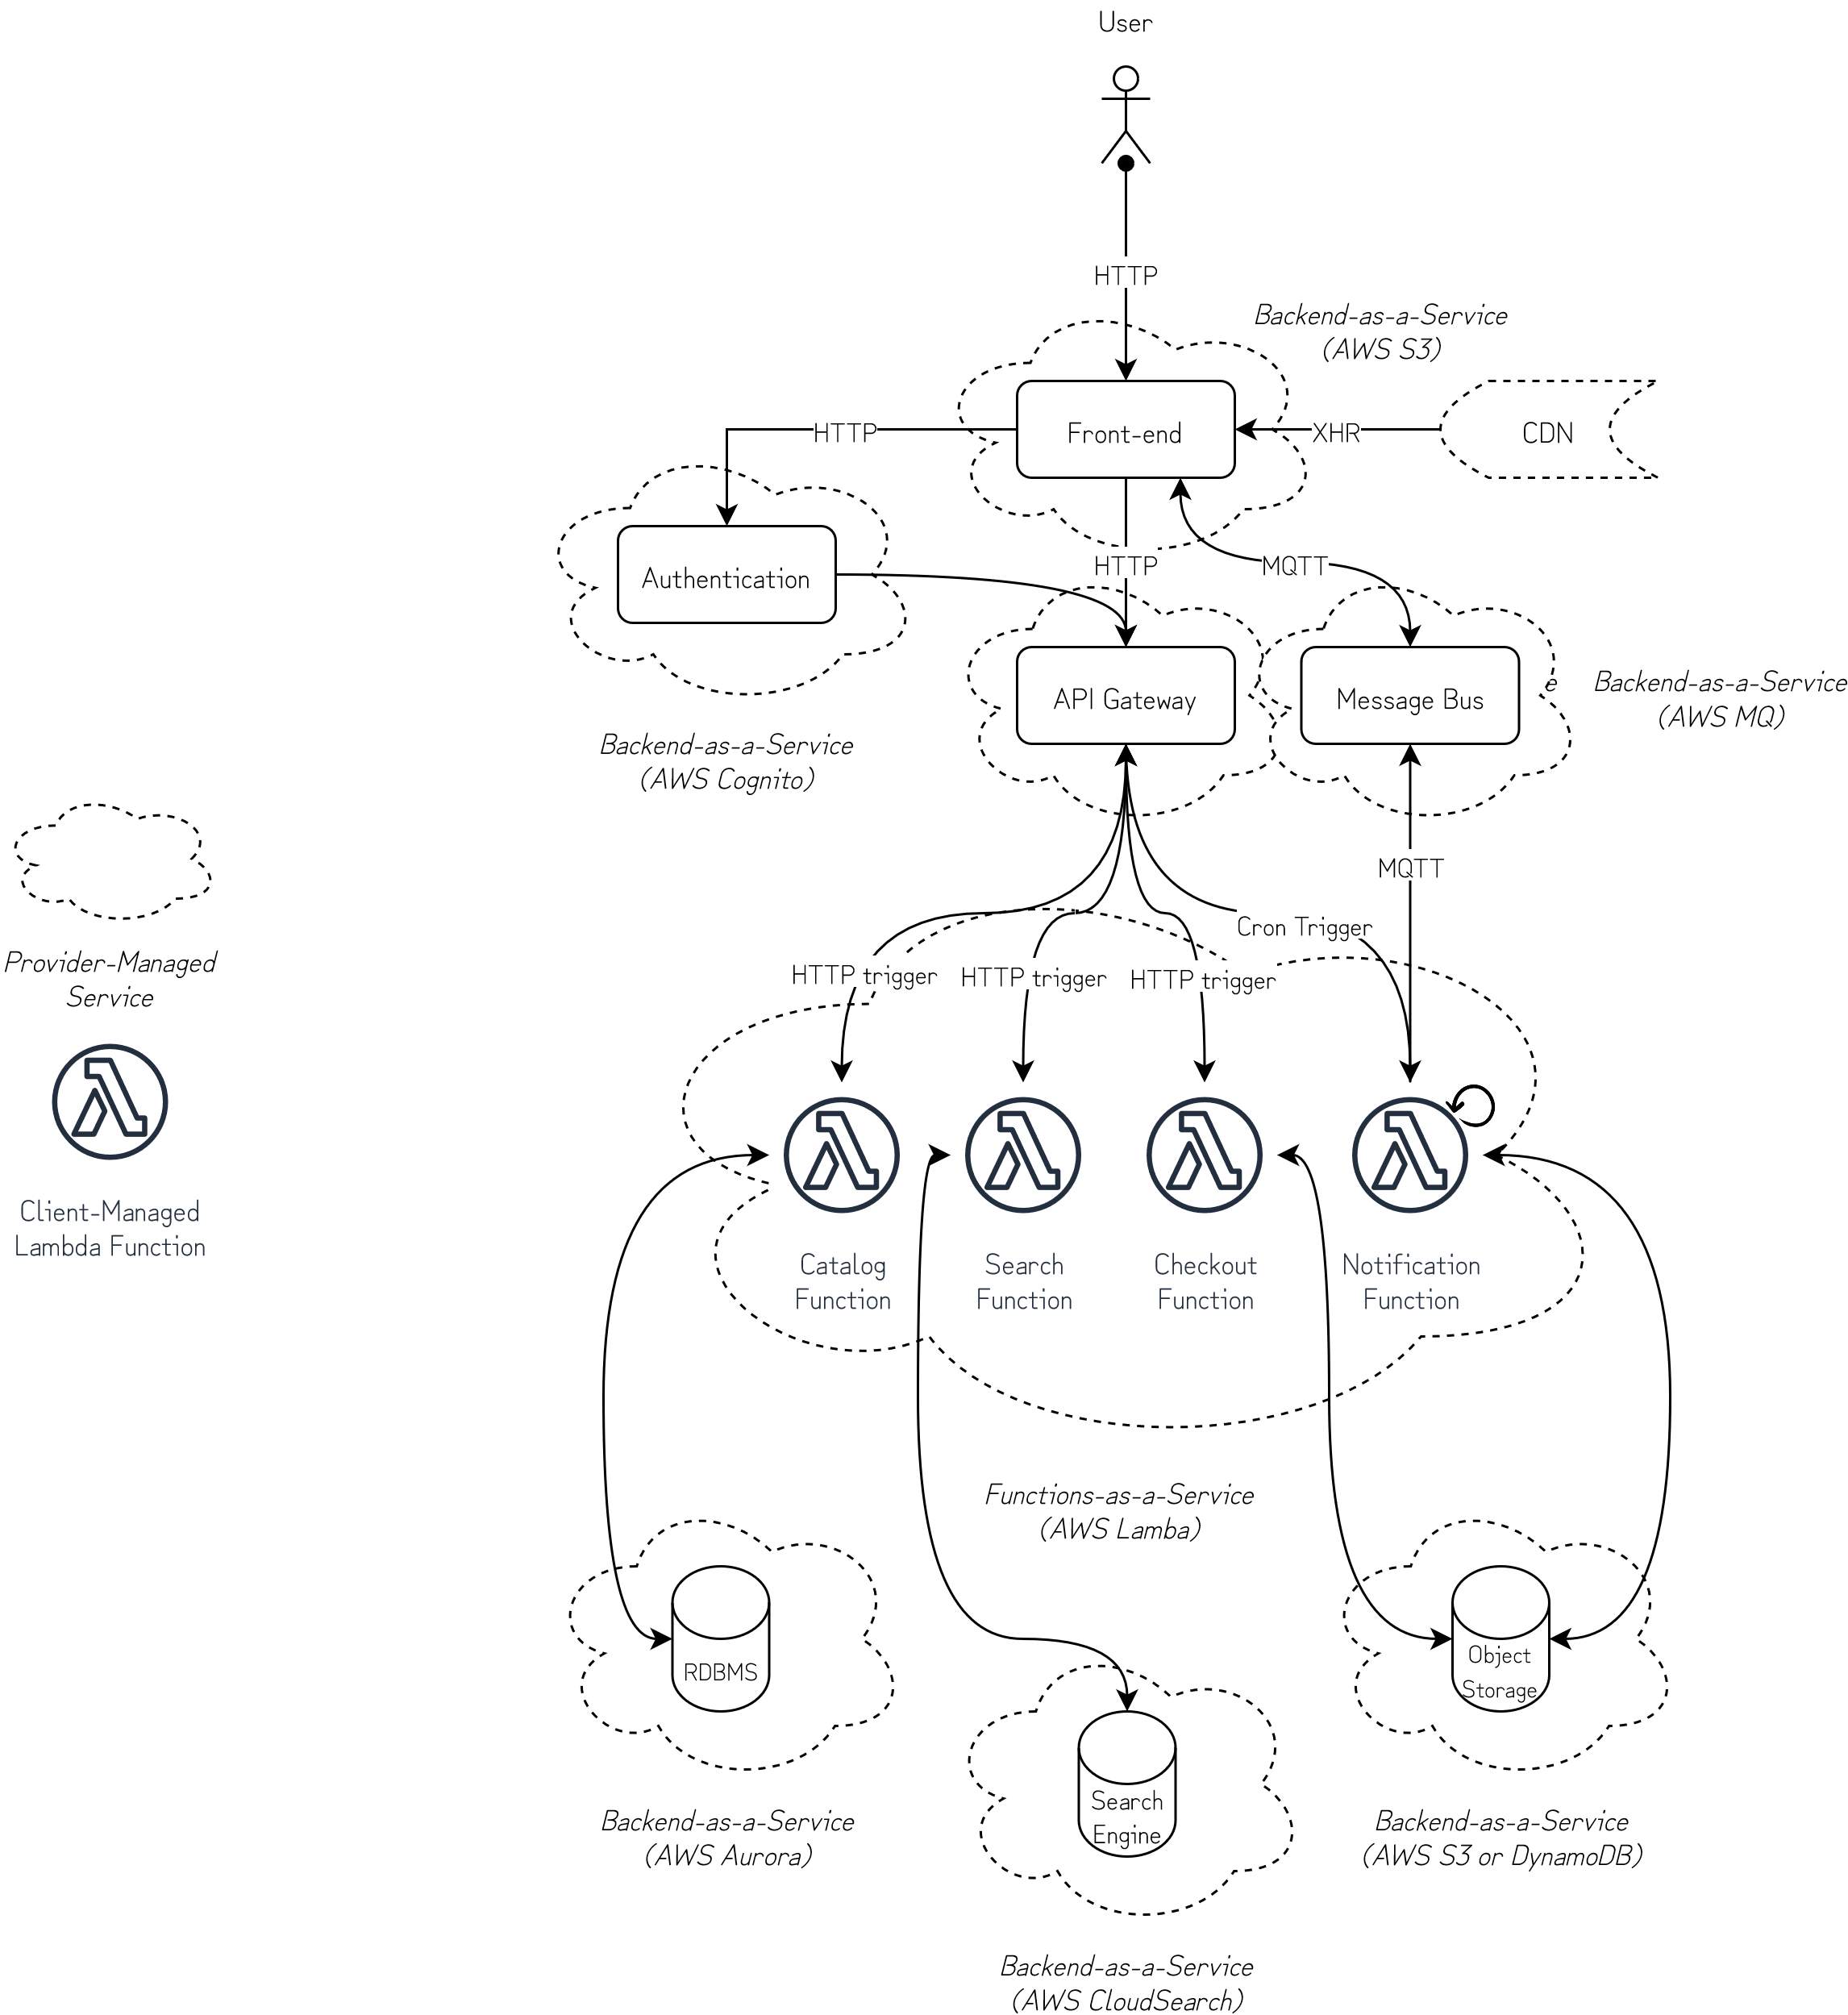
\includegraphics[width=\textwidth]{3_Chapitre1/figures/faas-web-app.png}
	\caption{Fictional reference architecture for a serverless e-commerce web application deployed in the Amazon Web Services ecosystem.}
	\label{fig:web-app}
\end{figure}

Dans les offres commerciales, serverless est généralement appelé \textit{Function as a Service} (FaaS). On a cru que les fonctions en tant qu'abstraction sur le cloud computing font partie d'une première génération d'offres serverless, et pourraient changer par la suite~\cite{hellersteinServerlessComputingOne2019}.

Serverless ne signifie pas que les serveurs ne sont plus utilisés pour héberger et exécuter des applications -- d'une manière similaire au PaaS, du point de vue du client, "serverless" fait référence à une abstraction sur les ressources matérielles qui permet aux ingénieurs de ne plus penser aux serveurs qui supportent leurs applications. Grâce aux mécanismes de mise à l'échelle automatique, ils n'ont pas à tenir compte du nombre optimal d'instances nécessaires pour exécuter leurs charges de travail dans le cadre d'une planification de la capacité. Les plateformes serverless sont conçues pour gérer les besoins de mise à l'échelle et répondre aux fluctuations de la demande, libérant ainsi les clients du fardeau d'avoir à définir des stratégies de mise à l'échelle explicites. Dans une vision stratifiée des déploiements cloud, le SPEC Research Group~\cite{spec-rg} présente une architecture de référence FaaS qui montre que le développement serverless permet aux développeurs d'être au plus près de la logique métier~\cite{vaneykSPECRGCloud2018, vaneykSPECRGReferenceArchitecture2019}.

Développer pour les plateformes serverless nécessite de repenser l'architecture d'une application. En effet, les serveurs dorsaux à longue durée de vie sont relégués aux solutions \textit{serverful} qui fournissent des serveurs toujours actifs~\cite{mateiTransitionServerfullServerless2020}, telles que les offres IaaS.

Comme l'ont souligné Shafiei et al.~\cite{shafieiServerlessComputingSurvey2021} dans leur enquête de 2022 sur l'informatique sans serveur, il n'existe pas de définition formelle du concept d'informatique sans serveur, bien que nous puissions identifier diverses différences essentielles entre les modèles serverful et serverless (résumées dans le tableau~\ref{table:serverful-serverless}).

Une différence majeure entre PaaS et FaaS est que FaaS permet une mise à l'échelle à zéro : les fournisseurs ne facturent les clients que lorsque leur application utilise effectivement des ressources matérielles, c'est-à-dire lorsque des fonctions sont exécutées sur la plateforme. Cela est possible parce que, dans le paradigme FaaS, les applications sont conçues comme une collection de microservices à courte durée d'exécution.

Les solutions Backend as a Service (BaaS) sont des offres commerciales et gérées de services backend, mises à la disposition des développeurs d'applications par le biais d'une API unifiée~\cite{mikeroberts2018serverless}. Les logiciels dorsaux consistent généralement en des services à état et à longue durée d'exécution qui ne peuvent pas être réduits à zéro. Afin de maintenir un modèle de tarification cohérent, les fournisseurs doivent proposer ces services de la même manière payante que les fonctions serverless. Ces services tiers constituent l'infrastructure de base des applications serverless en gérant l'état des fonctions déployées par les développeurs, par le biais, par exemple, de magasins de valeurs clés ou de stockage de fichiers ; en fournissant une authentification aux points d'extrémité de l'application ; en permettant les communications entre les fonctions à l'aide de bus de messages ; etc. La figure~\ref{fig:web-app} montre les dépendances possibles entre les fonctions serverless et les logiciels BaaS : l'application d'exemple s'appuie sur une authentification gérée par le fournisseur, un bus de messages, une base de données relationnelle, un moteur de recherche et un stockage d'objets, et l'utilisateur y accède par la passerelle API du fournisseur. Cette situation introduit un degré élevé de couplage entre l'application et les services spécifiques du fournisseur, ce qui risque de lier les développeurs à leur choix initial de fournisseur de services.

Serverless permet de réduire les frais généraux des développeurs en faisant abstraction de la gestion des serveurs, tout en permettant aux fournisseurs de partager les ressources physiques à un niveau de granularité très fin, ce qui permet d'obtenir une meilleure efficacité. Le niveau fin de granularité présenté dans le modèle FaaS permet au fournisseur d'offrir une élasticité parfaite : la mise à l'échelle et l'extension sont basées sur des événements, dans un modèle de tarification typique \textit{pay as you go}.

Cette abstraction permet aux fournisseurs de déployer du code dans plusieurs zones géographiques. Ce mécanisme de basculement garantit la disponibilité en cas de panne dans une zone de déploiement et réduit le risque de défaillance d'une fonction en cascade dans l'application~\cite{taibiPatternsServerlessFunctions2020}.

En outre, comme les instances de fonction sont créées à la demande par le fournisseur, le modèle de concurrence offert par les plateformes FaaS signifie que les performances d'une application peuvent évoluer linéairement avec le nombre de requêtes~\cite{mcgrathServerlessComputingDesign2017}.

\begin{table}[H]
    \caption{Comparison of key characteristics in serverless and serverful service models}
    \centering
    \begin{tabularx}{\textwidth} { 
      | >{\centering\arraybackslash}X 
      | >{\centering\arraybackslash}X 
      | >{\centering\arraybackslash}X  | }
         \hline
        \textit{Characteristic}  & \textit{Serverful} (IaaS, PaaS)           & \textit{Serverless} (FaaS)                                             \\ \hline
        Provisioning    & Customer responsibility          & Fully \textbf{managed} (\textit{i.e.} by the provider)    \\ \hline
        Billing         & Pay for \textbf{provisioned} resources    & Pay for \textbf{consumed} resources                                    \\ \hline
        Scaling         & Customer responsibility          & \textbf{autoscalinging} built in                                         \\ \hline
        Availability    & Depends on \textbf{provisioned} resources & Code runs in multiple high availability zones                 \\ \hline
        Fault tolerance & Depends on deployment strategy   & Backend services are fully \textbf{managed} and retries are guaranteed \\ \hline
        Concurrency     & Depends on \textbf{provisioned} resources & Virtually \textbf{infinite} \\
        \hline
    \end{tabularx}
    \label{table:serverful-serverless}
\end{table}

Divers auteurs (\cite{hellersteinServerlessComputingOne2019},~\cite{vaneykSPECRGCloud2018},~\cite{shafieiServerlessComputingSurvey2021},~\cite{khandelwalTaureauDeconstructingServerless2020}) considèrent déjà le serverless comme l'avenir du déploiement du cloud. Cependant, l'adoption du FaaS semble stagner parmi les développeurs de cloud~\cite{oreilly2020adoption}, et la Cloud Native Computing Foundation (CNCF) fait même état de chiffres en baisse~\cite{cncf2021report}.

\subsubsection{Charges de travail adaptées}

Dans son livre blanc de 2018~\cite{cncf2018whitepaper}, la Cloud Native Computing Foundation (CNCF) -- une initiative de la Fondation Linux soutenue par plus de 800 membres industriels impliqués dans les services cloud -- identifie des caractéristiques pour les cas d'utilisation serverless, notamment :

\begin{itemize}
    \item Charges de travail "étonnamment parallèles" : asynchrones et concurrentes, avec peu ou pas de communication et pas de synchronisation entre les processus ;
    \item Peu fréquentes avec des variations imprévisibles dans les exigences de mise à l'échelle, c'est-à-dire des tâches interactives ou événementielles plutôt que des tâches par lots ;
    \item Processus sans état et éphémères, sans besoin majeur d'un temps de démarrage instantané.
\end{itemize}

Nous pouvons affirmer que ces conditions sont trop restrictives pour l'informatique générale : par exemple, elles impliquent que les travaux de longue durée ne peuvent pas être mis en correspondance avec les déploiements FaaS. Les fournisseurs ont introduit des mécanismes tels que les fonctions d'étape ou les fonctions durables (\cite{aws-step-functions},~\cite{azure-durable-functions},~\cite{google-workflows}) pour mettre en œuvre des flux de travail serverless : une fonction d'orchestration maintient l'état à travers les fonctions sans état de l'application pour créer des flux de travail avec état~\cite{burckhardtNetheriteEfficientExecution}.

Les développeurs déploient déjà une partie de la logique de leurs applications vers des fonctions serverless. Selon une enquête~\cite{serverless2018survey} menée en 2018 par l'éditeur du framework Serverless auprès d'un panel de leurs utilisateurs, les exemples de cette logique incluent les pipelines de transformation de données, les plateformes d'alerte à haute disponibilité, les outils ETL (\textit{Extraire, Transformer, Charger}, la manipulation de données par lots), le transcodage de médias, etc. Ces applications sont un sous-ensemble de programmes informatiques qui produisent des résultats qui dépendent uniquement de l'entrée du programme : elles appliquent des transformations purement fonctionnelles aux données.

Les problèmes qui sont commodément divisés en lots de sous-tâches bénéficieraient également du niveau de concurrence virtuellement infini offert par le modèle serverless~\cite{golecIFaaSBusSecurityPrivacyBased2022}. Dans~\cite{agacheFirecrackerLightweightVirtualization}, les auteurs identifient des cas d'utilisation pour le serverless dans l'encodage vidéo à grande échelle, l'algèbre linéaire et la compilation parallèle.

Comme il existe des similitudes fondamentales entre une application architecturée en microservices et une application conçue pour un déploiement FaaS~\cite{jiaNightcoreEfficientScalable2021}, des applications à part entière peuvent être conçues avec FaaS à l'esprit. La figure~\ref{fig:web-app} donne un exemple d'architecture pour une application web de commerce électronique. La logique métier de l'application comprend trois fonctions serverless (catalogue, recherche et paiement) qui sont déclenchées par la navigation de l'utilisateur, et une fonction (notification) qui est ordonnancée pour s'exécuter périodiquement. Comme ces fonctions sont activées et désactivées en fonction de la charge de l'application, l'état doit être stocké dans un stockage persistant, c'est-à-dire une base de données relationnelle et un magasin d'objets qui sont tous deux gérés par le fournisseur. L'application s'appuie en outre sur des services gérés par le fournisseur : son moteur de recherche est alimenté par une solution BaaS, tout comme la fonction de notification et le mécanisme d'authentification.

En utilisant AWS Lambda en 2022, ce type d'application pourrait passer de zéro ressource utilisée à 150 To de RAM et 90 000 vCPU en moins de deux secondes~\cite{ionescu2022scaling}, ce qui permettrait de réagir rapidement aux variations de charge.

\subsubsection{Compromis dans les déploiements serverless}

Lorsque nous considérons le serverless comme un modèle de programmation, l'avantage immédiat est un coût de développement réduit pour les équipes qui s'appuient sur des offres BaaS : au lieu de mettre en œuvre des services backend internes tels que l'authentification ou les notifications, les développeurs se contentent d'introduire un boilerplate dans leur base de code de manière à connecter les applications frontales aux API BaaS de leur fournisseur de cloud. Toutefois, ce degré de couplage signifie que les développeurs peuvent se retrouver enfermés dans un environnement spécifique à un fournisseur, perdant en fin de compte le contrôle des coûts de déploiement~\cite{baarziMeritsViabilityMultiCloud2021}.

Du point de vue du client, le FaaS associé au BaaS géré permet une mise à l'échelle parfaite. Les clients sont facturés au plus juste, uniquement lorsque les ressources sont effectivement utilisées et pour la durée exacte de l'exécution. Du point de vue du fournisseur, l'augmentation du nombre de locataires permet un meilleur multiplexage des ressources, ce qui se traduit par une efficacité accrue et donc des bénéfices plus importants. Ce mécanisme d'autoscalinging a un coût en termes de latence : faire tourner de nouveaux bacs à sable pour les requêtes entrantes peut créer des situations de \textit{démarrages à froid} où les temps d'initialisation dominent les temps d'exécution des fonctions~\cite{Jiang2021TowardsDS}. L'autoscalinging serverless a d'autres implications en termes de débit : étant donné que l'état des fonctions doit être persisté dans un stockage désagrégé, les applications qui affichent des modèles de communications étendues entre les fonctions peuvent souffrir du temps d'expédition des données vers les nœuds de calcul~\cite{mullerLambadaInteractiveData2020}.

Un effet secondaire du modèle FaaS est l'augmentation du nombre de tâches par client. Bien que l'augmentation de la concurrence, de la densité et de l'utilisation des ressources soit un argument de vente pour les fournisseurs de FaaS et les clients, ces travaux de courte durée doivent être isolés les uns des autres pour éviter la fuite de secrets entre les clients, ou à l'échelle d'une application unique comprenant plusieurs fonctions individuelles~\cite{vaqueroLockingSkySurvey2011}.

\begin{table}[H]
    \caption{Considerations regarding the FaaS service model}
    \centering
    \begin{tabularx}{\textwidth} { 
      | >{\centering\arraybackslash}X 
      | >{\centering\arraybackslash}X  | }
     \hline
        \textit{Pros} & \textit{Cons} \\ \hline
        Reduced \textbf{development costs} for teams leaning on BaaS offerings & Can we map \textbf{any application} to the FaaS architecture? \\ \hline
        Reduced \textbf{costs in operations} thanks to fully managed infrastructure & Risks of \textbf{vendor lock-in} due to high degree of coupling with BaaS offerings \\ \hline
        \textbf{Perfect scaling} allows billing granularity close to actual use of resources & Increase in \textbf{latency} due to cold starts, and decreased \textbf{throughput} from communications through slow storage to handle statefulness \\ \hline
        Providers can achieve \textbf{better efficiency} in resources multiplexing leading to increased profits & Massive multitenancy might involve \textbf{security} threats \\ \hline
    \end{tabularx}
    \label{table:serverless-tradeoffs}
\end{table}

Pour tirer parti des atouts du modèle, les clients et les fournisseurs doivent tenir compte des compromis associés aux déploiements serverless. Le tableau~\ref{table:serverless-tradeoffs} résume les principaux points à prendre en compte lors de l'utilisation de serverless pour déployer des applications dans le cloud.

\section{Conclusion}
